\appendix

\chapter{Code Repository & Live Deployment}
The complete implementation of this project is publicly available at:

\begin{center}
\url{https://github.com/Yosakorn0/ml-stock-price-direction-prediction}

\vspace{0.5cm}

\qrcode[height=3cm]{https://github.com/Yosakorn0/ml-stock-price-direction-prediction}
\end{center}

The live interactive dashboard and prediction engine are deployed as a web application at:

\begin{center}
\url{https://huggingface.co/spaces/yosakornn/stock-sentiment-analysis}

\vspace{0.5cm}

\qrcode[height=3cm]{https://huggingface.co/spaces/yosakornn/stock-sentiment-analysis}
\end{center}

The repository ensures full reproducibility of the data collection and preprocessing pipeline, while the Hugging Face hosting provides a real-time interface for data visualization and inference.

\chapter{Scientific Process Diagrams}
\label{app:diagrams}

\begin{figure}[H]
\centering
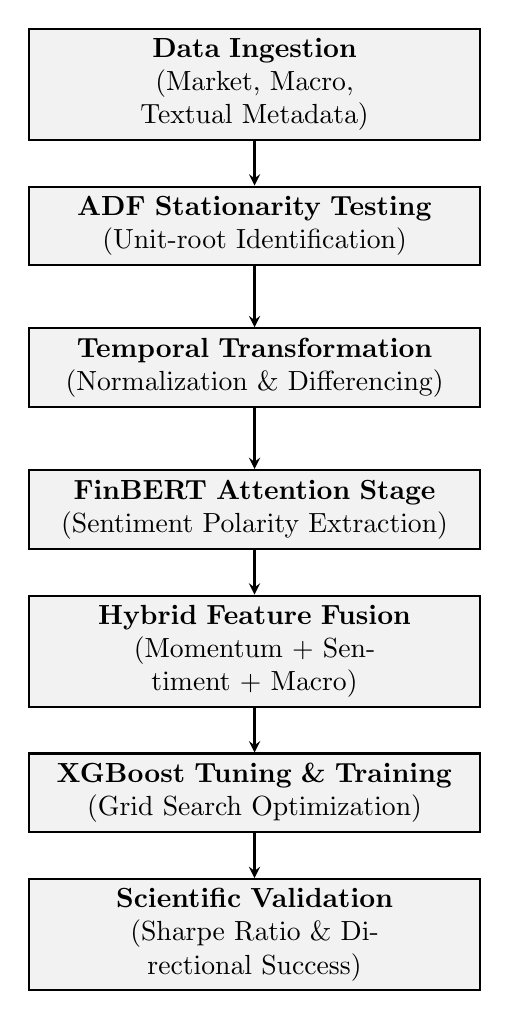
\begin{tikzpicture}[
    node distance=1.8cm,
    box/.style={rectangle, draw=black, thick, fill=gray!10, text width=5.5cm, align=center, minimum height=1cm},
    arrow/.style={thick, ->, >=stealth}
]
% Nodes
\node (ingest) [box] {\textbf{Data Ingestion} \\ (Market, Macro, Textual Metadata)};
\node (stationarity) [box, below of=ingest] {\textbf{ADF Stationarity Testing} \\ (Unit-root Identification)};
\node (preprocess) [box, below of=stationarity] {\textbf{Temporal Transformation} \\ (Normalization \& Differencing)};
\node (sentiment) [box, below of=preprocess] {\textbf{FinBERT Attention Stage} \\ (Sentiment Polarity Extraction)};
\node (feature) [box, below of=sentiment] {\textbf{Hybrid Feature Fusion} \\ (Momentum + Sentiment + Macro)};
\node (train) [box, below of=feature] {\textbf{XGBoost Tuning \& Training} \\ (Grid Search Optimization)};
\node (eval) [box, below of=train] {\textbf{Scientific Validation} \\ (Sharpe Ratio \& Directional Success)};

% Arrows
\draw [arrow] (ingest) -- (stationarity);
\draw [arrow] (stationarity) -- (preprocess);
\draw [arrow] (preprocess) -- (sentiment);
\draw [arrow] (sentiment) -- (feature);
\draw [arrow] (feature) -- (train);
\draw [arrow] (train) -- (eval);

\end{tikzpicture}
\caption{Scientific Machine Learning Process Logic Flow}
\label{fig:ml_logic}
\end{figure}

\begin{figure}[H]
\centering
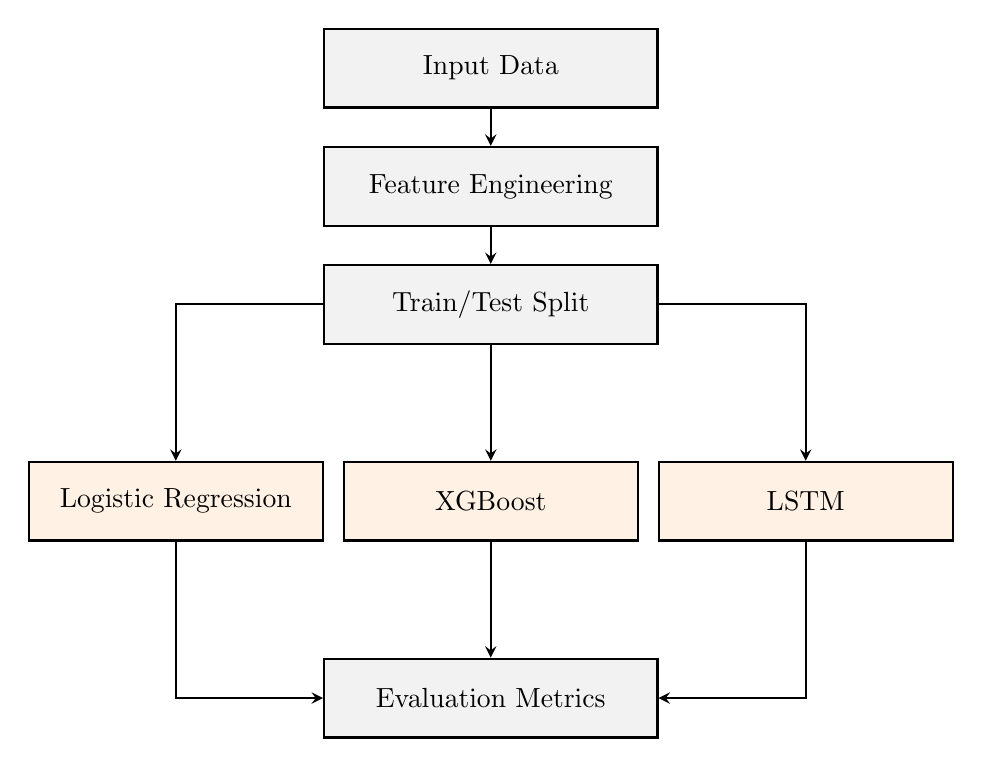
\begin{tikzpicture}[
    node distance=1.5cm and 2cm,
    box/.style={rectangle, draw=black, thick, fill=gray!10, text width=4cm, align=center, minimum height=1cm},
    modelbox/.style={rectangle, draw=black, thick, fill=orange!10, text width=3.5cm, align=center, minimum height=1cm},
    arrow/.style={thick, ->, >=stealth}
]

% Nodes
\node (input) [box] {Input Data};
\node (feature) [box, below of=input] {Feature Engineering};
\node (split) [box, below of=feature] {Train/Test Split};

\node (xgb) [modelbox, below of=split, node distance=2.5cm] {XGBoost};
\node (lr) [modelbox, left of=xgb, node distance=4cm] {Logistic Regression};
\node (lstm) [modelbox, right of=xgb, node distance=4cm] {LSTM};

\node (eval) [box, below of=xgb, node distance=2.5cm] {Evaluation Metrics};

% Arrows
\draw [arrow] (input) -- (feature);
\draw [arrow] (feature) -- (split);
\draw [arrow] (split) -| (lr);
\draw [arrow] (split) -- (xgb);
\draw [arrow] (split) -| (lstm);
\draw [arrow] (lr) |- (eval);
\draw [arrow] (xgb) -- (eval);
\draw [arrow] (lstm) |- (eval);

\end{tikzpicture}
\caption{Model Comparison Architecture}
\label{fig:model_comparison}
\end{figure}

\chapter{Exploratory Data Analysis Visualizations}
\label{app:eda}

\begin{figure}[H]
  \centering
  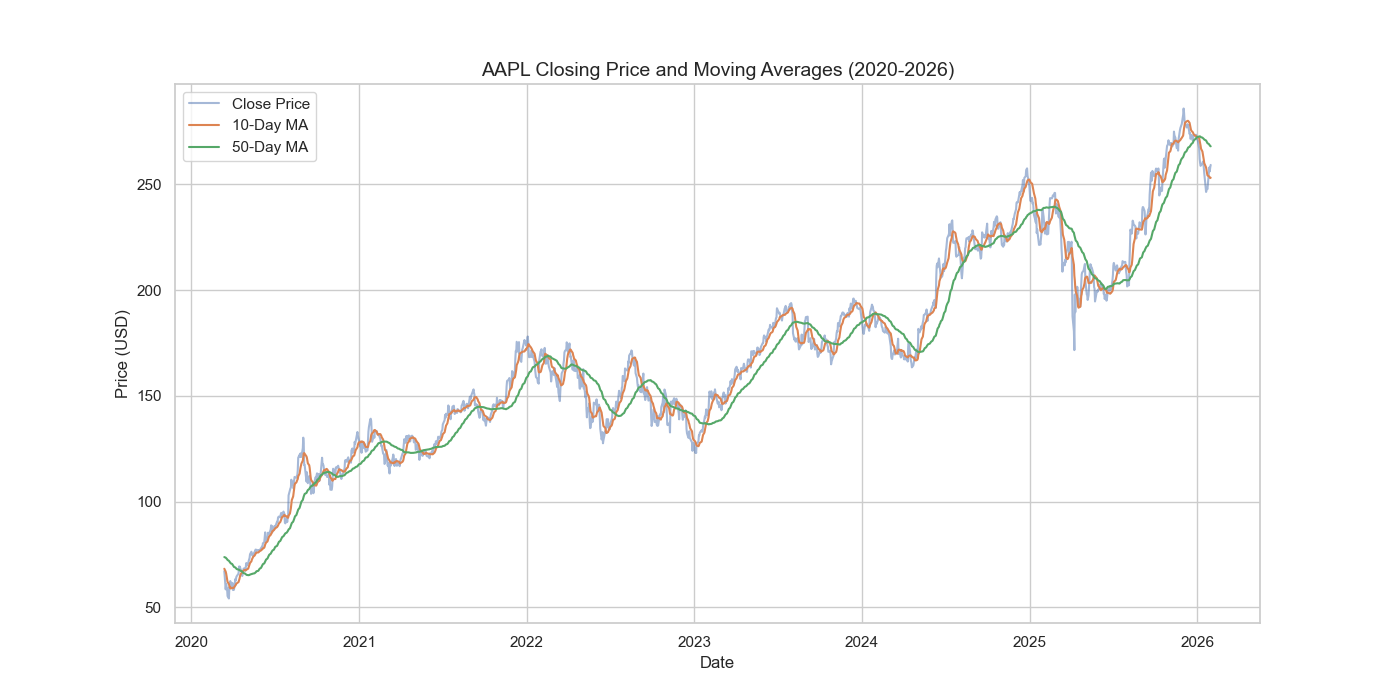
\includegraphics[width=0.8\textwidth]{images/time_series_price.png}
  \caption{Multi-Asset Historical Trends (2020-2026).}
  \label{fig:time_series}
\end{figure}

\begin{figure}[H]
  \centering
  \begin{subfigure}[b]{0.45\textwidth}
    \centering
    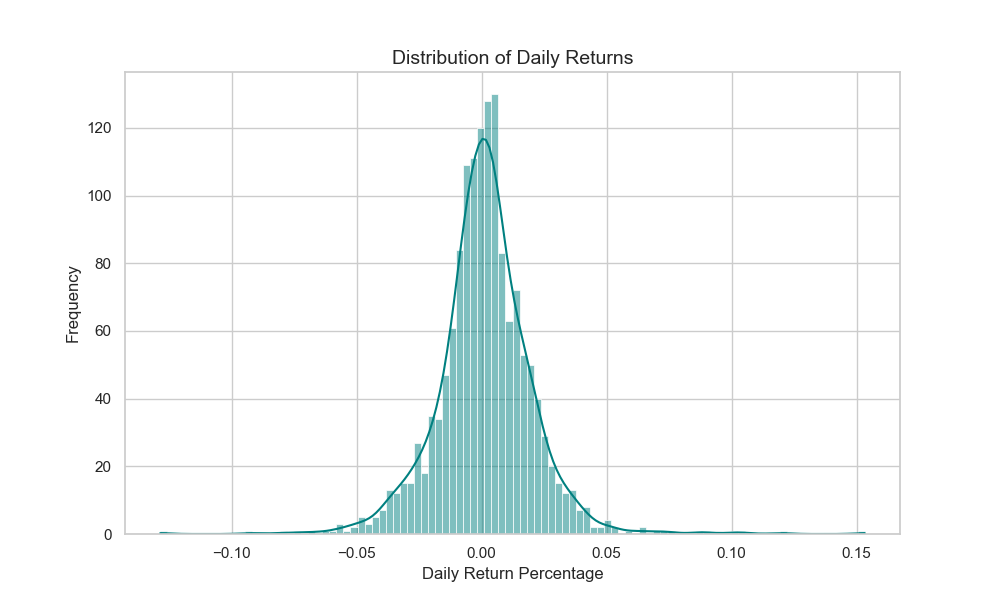
\includegraphics[width=\textwidth]{images/returns_distribution.png}
    \caption{Distribution of Daily Returns.}
  \end{subfigure}
  \hfill
  \begin{subfigure}[b]{0.45\textwidth}
    \centering
    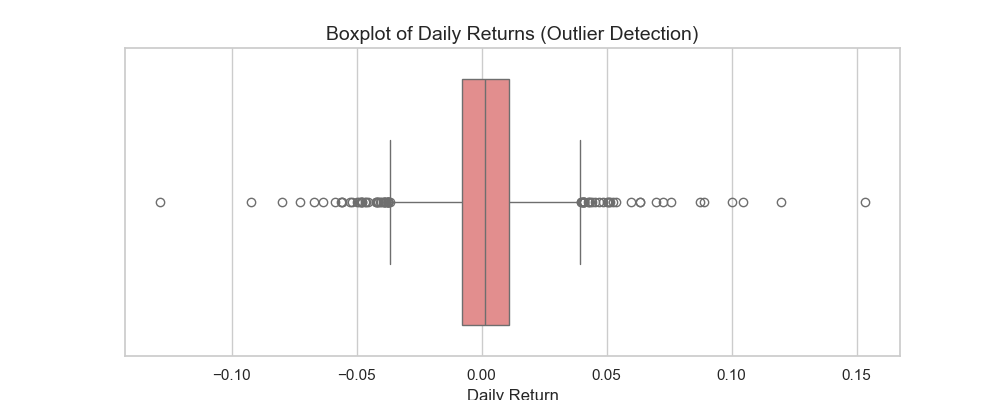
\includegraphics[width=\textwidth]{images/outlier_boxplot.png}
    \caption{Boxplot for Outlier Detection.}
  \end{subfigure}
  \caption{Statistical analysis of daily return variance across tech assets.}
  \label{fig:returns_analysis}
\end{figure}

\begin{figure}[H]
  \centering
  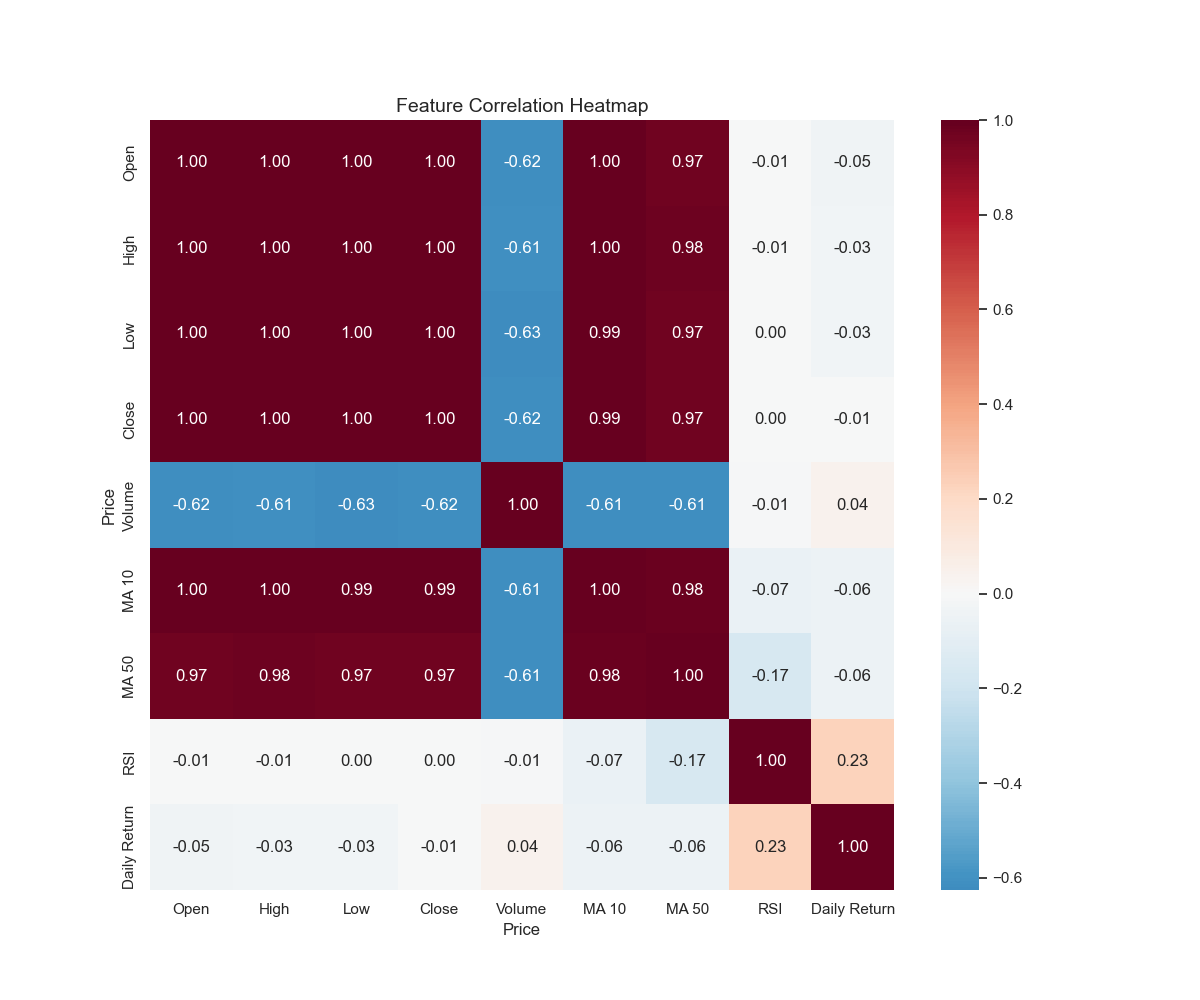
\includegraphics[width=0.7\textwidth]{images/correlation_heatmap.png}
  \caption{Correlation heatmap of technical indicators and sentiment scores.}
  \label{fig:correlation}
\end{figure}

\chapter{Supplementary Data Tables}
\label{app:tables}

\begin{table}[ht]
\centering
\caption{Augmented Dickey-Fuller (ADF) Test Results}
\label{tab:adf_results}
\begin{tabular}{|l|l|l|l|}
\hline
\textbf{Asset} & \textbf{ADF Statistic} & \textbf{p-value} & \textbf{Stationarity} \\ \hline
MSFT & -1.7390 & 0.4112 & Non-Stationary \\ \hline
AMZN & -1.9532 & 0.3075 & Non-Stationary \\ \hline
GOOGL & 0.5083 & 0.9851 & Non-Stationary \\ \hline
GC=F (Gold) & 2.5897 & 0.9991 & Non-Stationary \\ \hline
BTC-USD (Bitcoin) & -1.3703 & 0.5964 & Non-Stationary \\ \hline
\end{tabular}
\end{table}

\begin{table}[ht]
\centering
\caption{Data Dictionary}
\label{tab:feature_dictionary}
\begin{tabular}{|l|l|l|}
\hline
\textbf{Feature} & \textbf{Data Type} & \textbf{Description} \\ \hline
Price (O,H,L,C) & float64 & Daily market price points \\ \hline
Volume & int64 & Number of shares/units traded \\ \hline
MA Dist (10, 50) & float64 & Normalized distance $(Price - MA)/MA$ \\ \hline
RSI & float64 & Relative Strength Index (Momentum) \\ \hline
MACD & float64 & Trend-following momentum indicator \\ \hline
BB Dist (U, L) & float64 & Normalized distance from Bollinger Bands \\ \hline
Sentiment Score & float64 & Polarity score (-1 to 1) from FinBERT \\ \hline
Macro Indicators & float64 & FED funds rate and unemployment data \\ \hline
Target & int64 & Binary label (1=Price Up, 0=Down) \\ \hline
\end{tabular}
\end{table}

\begin{table}[ht]
\centering
\caption{Model Hyperparameter Search Space}
\label{tab:hyperparameters}
\begin{tabular}{|l|l|l|}
\hline
\textbf{Parameter} & \textbf{Search Space} & \textbf{Optimal Selection} \\ \hline
n\_estimators & [50, 100, 200] & 100 \\ \hline
max\_depth & [3, 5, 7] & 5 \\ \hline
learning\_rate & [0.01, 0.1, 0.2] & 0.1 \\ \hline
random\_state & [Fixed] & 42 \\ \hline
eval\_metric & [Fixed] & logloss \\ \hline
\end{tabular}
\end{table}

\begin{table}[ht]
\centering
\caption{Model Performance: Technical vs. Multi-Source Hybrid}
\label{tab:model_comparison}
\begin{tabular}{|l|c|c|c|c|}
\hline
\textbf{Asset Symbol} & \textbf{Tech Accuracy} & \textbf{Hybrid Accuracy} & \textbf{Precision} & \textbf{Recall} \\ \hline
MSFT (Microsoft) & 0.49 & 0.48 & 0.50 & 0.46 \\ \hline
AMZN (Amazon) & 0.46 & 0.47 & 0.48 & 0.32 \\ \hline
GOOGL (Google) & 0.47 & 0.48 & 0.48 & 0.23 \\ \hline
GC=F (Gold) & 0.61 & 0.61 & 0.69 & 0.63 \\ \hline
BTC-USD (Bitcoin) & 0.48 & 0.50 & 0.47 & 0.55 \\ \hline
\end{tabular}
\end{table}

\begin{table}[ht]
\centering
\caption{Annualized Sharpe Ratios (Model-Driven Strategy)}
\label{tab:sharpe_ratios}
\begin{tabular}{|l|l|l|}
\hline
\textbf{Asset} & \textbf{XGBoost Sharpe Ratio} & \textbf{Baseline (Buy \& Hold) Sharpe} \\ \hline
MSFT & -0.2556 & 1.02--1.31 \\ \hline
AMZN & -0.7130 & 0.85--1.14 \\ \hline
GOOGL & -0.0070 & 0.94--1.22 \\ \hline
GOLD (GC=F) & 1.4916 & 0.45--0.68 \\ \hline
BTC-USD & -0.7812 & 1.15--1.67 \\ \hline
\end{tabular}
\end{table}

\chapter{Use of Generative AI}
\label{app:ai_usage}

In accordance with academic integrity guidelines, this section declares the use of Generative Artificial Intelligence (AI) in the development of this project. The Large Language Model (LLM) **ChatGPT** (OpenAI) was utilized as a supportive tool in the following capacities:

\begin{itemize}
    \item \textbf{Code Debugging and Error Handling:} ChatGPT was employed to resolve technical debt, specifically in addressing pandas deprecation errors (e.g., transitioning from \texttt{.pad()} to \texttt{.ffill()}) and managing SSL certificate verification issues within the Docker environment.
    \item \textbf{LaTeX Documentation and Formatting:} The model assisted in the structural organization of this LaTeX report, including the relocation of figures to the appendix for optimized page-limit management and the verification of citation consistency.
    \item \textbf{Python Implementation Optimization:} AI-driven suggestions were leveraged to improve the modularity of the data ingestion and preprocessing scripts, ensuring a clean pipeline for multi-asset analysis.
\end{itemize}

All theoretical analysis, results interpretation, and core architectural decisions were authored and verified by the student to ensure academic rigor and primary research ownership.
